\documentclass[12pt, a4paper]{article}
\usepackage[utf8]{inputenc}

% Format
\usepackage{layout}
\setlength{\parindent}{0.5in}
\setcounter{secnumdepth}{0}
\usepackage{lineno}
\usepackage{authblk}

% Font
\usepackage{MinionPro}
\input glyphtounicode
\pdfgentounicode=1
\usepackage{microtype}
\usepackage[super]{nth}

% Language
\usepackage[british]{babel}

% References
\usepackage[nosectionbib, tocbib, unnumberedbib]{apacite}

% Figures
\usepackage{graphicx}
\usepackage[small, labelfont=it, labelsep=period]{caption}

% Tables
\usepackage{booktabs}
\usepackage{tabularx}

% Commands
\newcommand{\pest}[4]{$ \text{Pr} (\text{``us''} | \text{#1}) = #2$, $[#3, #4]$}
\newcommand{\pdif}[4]{$ \Delta\text{Pr} (\text{``us''} | \text{#1}) = #2$, $[#3, #4]$}

% Frontmatter
\title{Intergroup contact fosters\\more inclusive social identities}
\date{November 5, 2018}
\author{Nils Karl Reimer}
\author[2]{Shanmukh V. Kamble}
\author[3]{Katharina Schmid}
\author[1]{Miles Hewstone}
\affil[1]{University of Oxford}
\affil[2]{Karnatak University, Dharwad}
\affil[3]{ESADE Business School, Ramon Llull University}
\renewcommand\Affilfont{\small}

\begin{document}

\maketitle

\begin{abstract}
\noindent We examined how people construct their social identities from multiple group memberships---and whether intergroup contact can reduce bias by fostering more inclusive social identities. South Indian participants ($N = 351$) from diverse caste backgrounds viewed 24 identity cards, each representing a person with whom participants shared none, one, two, or all of three group memberships (caste, religion, nationality). Participants judged each person as ``us'' or ``not us'', showing whom they included in their ingroup, and whom they excluded.  Participants tended to exclude caste and religious minorities, replicating persistent social divides. Bridging these divides, cross-group friendship was associated with more inclusive identities which, in turn, were associated with more favourable outgroup attitudes. Negative contact was associated with less inclusive identities, showing that past experiences shaped whom participants considered ``us'' or ``not us''. Contact and identity processes were unrelated to support for affirmative action in advantaged and disadvantaged caste groups.\\[1ex]
\noindent \textbf{Keywords:} intergroup contact, social identity, multiple categorization, intergroup relations, affirmative action \\[1ex]
\end{abstract}

\linenumbers

\noindent (for a review, see \citeNP{authors_theories_inpress}) (see Figure~\ref{fig:f1}) \cite{devos_american_2005}

\begin{figure}
\centering
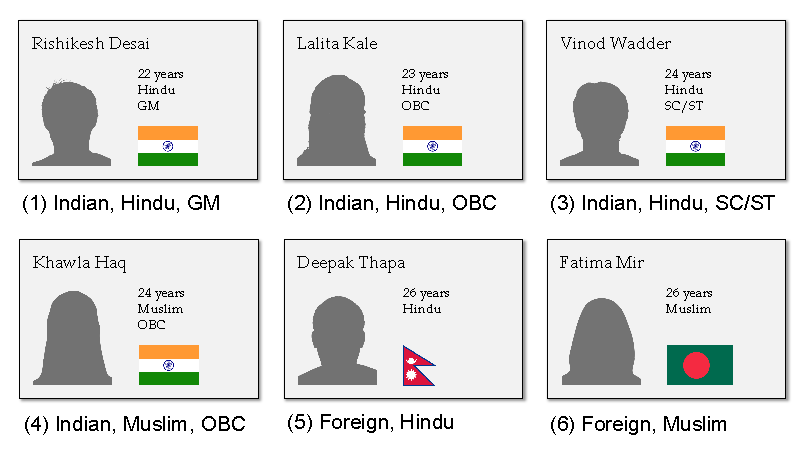
\includegraphics[scale=1]{../figures/figure-1}
\caption{
Schematic representations of social identity structures, ordered by social identity inclusiveness \protect\fullcite{dommelen_construing_2015}. Shaded regions represent the groups which a participant has to categorize as ``us'' to be assigned that structure. An Indian Hindu, for example, may consider only people who share their nationality, religion, and caste as ingroup members (intersection). Someone else may consider all their fellow Indians, whatever their religion or caste, as ingroup members (dominance). Another person may consider anyone who shares their nationality or religion as ingroup members (merger).
}
\label{fig:f1}
\end{figure}

\nolinenumbers

\bibliographystyle{apacite}
\bibliography{references}

\end{document}